\section{Data structures for $hp$-adaptivity}
\label{sec:data_structures}
The need for mesh adaptivity brings further demands that must be
taken into account in the design of the data structures. A tree-like
hierarchy of element refinement levels must be introduced and also
more complicated neighbor search algorithms are required to correctly
initialize the edge and vertex nodes and the integration points on the edges. The complexity of the data
structures reflects strongly on the complexity of the rest of the
finite element code. 

Simplifying assumptions, such as the
$k$-irregularity rules, are often imposed on the mesh with the aim of reducing code complexity.
However, these assumptions can deteriorate the numerical performance of the code.

In the following we present an original design of data structures for
adaptive meshes, free of any regularity assumptions yet retainign
extreme simplicity.

Calculation of fluxes in DGFEM with arbitrary-level hanging will also be described.

\subsection{Node and element structures}

It should be noted first that we have departed from traditional mesh
data structures storing complete information about the finite element
problem. Our mesh structures contain geometrical information only. The remaining data, including basis function indices, boundary conditions,
polynomial degrees, etc., are stored in separate structures describing
concrete finite element spaces ($H^1$, \Hcurl, ...) and are accessible
via the identification numbers of nodes and elements. This was done to allow
multiple spaces and multiple element types to co-exist on the same mesh,
which is vital for solving multi-physics and coupled problems. See~\cite{my presentation somewhere on my web or what not}

The entire mesh is defined by two arrays of the following C structures.
The first one stores all nodes:
\begin{lstlisting}
  structure Node
  {
    // Type of the Node - either vertex, or edge.
    type;

    // Identificator of the particular Node.
    int id;

    // Physical coordinates of this Node, in case it is a vertex Node.
    coordinate x;
	 coordinate y;

    // Two neighboring elements of this Node, in case it is an edge Node.
	 Element elements[2];
  };
\end{lstlisting}

This structure defines both vertex and edge nodes by utilizig the 
construct to distinguish between an edge and a vertex node. The standard vertex positions {\tt x}, {\tt y},
while typically stored separately, were placed in the vertex variant
of the {\tt Node} structure for simplicity. 
The edge variant contains pointers to the two elements
sharing the edge node (useful eg. when looking for a neighbor of an element sharing a particular edge in order to calculate the numerical flux across the edge).

The member {\tt type} determines the variant of the 
structure. The remaining members are omitted for simplicity.

Elements are defined by the second structure:

\begin{lstlisting}
  struct Element
  {
    // Type of the Element - either triangle, or quadrilateral.
    type;

    // Identificator of the particular Element.
    int id;

	 // Info whether this element is active (has not been refined further).
    boolean active;

    // vertex nodes
    Node vn[4];

    // edge nodes
    Node en[4];
  };
\end{lstlisting}

An element can be either active or inactive, hence the one-bit variable
{\tt active}. Active elements store pointers to the appropriate vertex
and edge nodes. Inactive elements are those which have been split and
are excluded from the computation. Their purpose is to hold pointers
to the descendant elements.

Triangular and quadrilateral elements share the same structure and are
distinguished by the member {\tt type}. The rest of the variables are analogous
to the {\tt Node} structure.

\subsection{Eliminating neighbor search by hashing}
\label{sec:hash}

To properly initialize edge node pointers after reading a mesh file,
one has to construct neighbor lists for all elements and use them in
such a way that only one node is created for each edge. Further
problems arise when certain elements are refined after automatic mesh
adaptation. Unless hanging nodes are removed by extra refinements, no
longer is each edge shared by at most two elements (there can be more of them). Standard neighbor
lists fail to fully capture such situations and thus more complex
data structures, eg. trees \cite{demk1}, have to be introduced.

Loosely inspired by \cite{skala}, we have avoided all of these problems
by introducing a function which, given the {\tt id} numbers of two nodes,
returns a pointer to the node halfway between them. If no such node
exists, it is created first. The task of translating two numbers to
a node pointer is accomplished using a hash table.

We are maintaining two independent layers of nodes: the first layer
contains all vertex nodes, the second all edge nodes. The following
two functions can be called:

\begin{lstlisting}
  Node* get_vertex_node(int id1, int id2);
  Node* get_edge_node(int id1, int id2);
\end{lstlisting}

All nodes, apart from being accessible by their {\tt id} number, can be reached using these functions by
passing the {\tt id}s of their ``parent'' nodes. Top-level vertex nodes (those loaded from the mesh file)
are stored at the beginning of the node array and can be accessed directly without hashing. Mesh
initialization then becomes trivial:

\begin{lstlisting}
  for all Elements
    vertex_numbers = read element vertex id numbers
    for all edges of the Element
      Element.vn = vertex_numbers
      Element.en[0] = get_edge_node(vertex_numbers[0], vertex_numbers[1]);
      Element.en[1] = get_edge_node(vertex_numbers[1], vertex_numbers[2]);
      Element.en[2] = get_edge_node(vertex_numbers[2], vertex_numbers[3]);
      // In case of triangles
      Element.en[3] = get_edge_node(vertex_numbers[3], vertex_numbers[0]);
    }
  }
\end{lstlisting}

Element refinement is also very straightforward. No care must be taken of the neighboring
elements, regardless of their refinement level or even existence:

\begin{lstlisting}
  create_triangle(Node v0, Node v1, Node v2)
  {
    Element e;
    e.vn[0] = v0;
    e.vn[1] = v1;
    e.vn[2] = v2;
    e.en[0] = get_edge_node(v0.id, v1.id);
    e.en[1] = get_edge_node(v1.id, v2.id);
    e.en[2] = get_edge_node(v2.id, v0.id);
  }
  
  void refine_triangle(Element e)
  {
    Node x0 = get_vertex_node(e.vn[0].id, e.vn[1].id);
    Node x1 = get_vertex_node(e.vn[1].id, e.vn[2].id);
    Node x2 = get_vertex_node(e.vn[2].id, e.vn[0].id);
    e.sons[0] = create_triangle(e.vn[0], x0, x2);
    e.sons[1] = create_triangle(x0, e.vn[1], x1);
    e.sons[2] = create_triangle(x2, x1, e.vn[2]);
    e.sons[3] = create_triangle(x0, x1, x2);
    e.active = 0;
  }

  create_quad(Node v0, Node v1, Node v2)
  {
    Element e;
    e.vn[0] = v0;
    e.vn[1] = v1;
    e.vn[2] = v2;
    e.vn[3] = v3;

    e.en[0] = get_edge_node(v0.id, v1.id);
    e.en[1] = get_edge_node(v1.id, v2.id);
    e.en[2] = get_edge_node(v2.id, v3.id);
    e.en[3] = get_edge_node(v3.id, v0.id);
  }
  
  void refine_quad(Element e)
  {
    Node x0 = get_vertex_node(e.vn[0].id, e.vn[1].id);
    Node x1 = get_vertex_node(e.vn[1].id, e.vn[2].id);
    Node x2 = get_vertex_node(e.vn[2].id, e.vn[3].id);
    Node x3 = get_vertex_node(e.vn[3].id, e.vn[0].id);
    e.sons[0] = create_quad(e.vn[0], x0, mid, x3);
    e.sons[1] = create_quad(x0, e.vn[1], x1, mid);
    e.sons[2] = create_quad(mid, x1, e.vn[2], x2);
    e.sons[3] = create_quad(x3, mid, x2, e.vn[3]);
    e.active = 0;
  }
\end{lstlisting}

Each hash table is implemented as an array of linked lists. 
This hash table organization has the advantage of simple node
removal, which is required if a node is no longer needed by any element.

\subsection{Finding all neighbors of an element}
In element-wise assembling procedure with arbitrary-level hanging nodes, when calculating fluxes across mesh edges, one needs values from both sides of the edge. To achieve this, the integration points need to be matched correctly, and proper values in these points from the adjacent element need to be extracted for all involved functions defined on the mesh (basis functions, previous time level solutions). This is not easy to manage. A simplified version of the algorithm is in Appendix 1.

\subsection{Determining node type}

Figure \ref{fig_nodes} shows a simple mesh with hanging nodes. 
Five types of nodes can be identified: standard vertex nodes (A), 
standard edge nodes (B), constrained vertex nodes (C), constrained
edge nodes (D) and finally standard edge nodes and constrained
vertex nodes at the same place (E).

\begin{figure}[H]
  \centering
  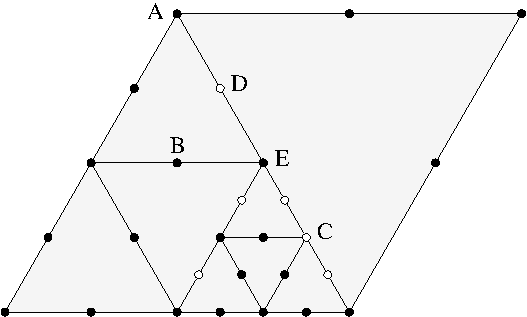
\includegraphics[width=0.55\textwidth]{img/nodes.pdf}
  \caption{Mesh with hanging nodes}
  \label{fig_nodes}
\end{figure}

As the elements in the mesh get refined (or derefined), some
nodes are created, others are removed and some change their types.
One has to be able to quickly recognize whether a node is constrained
or unconstrained without searching in the element hierarchy.
This is achieved through the member {\tt ref} of the structure {\tt Node}.
At all times this variable holds the number of elements pointing
to the node. This is the reason why all nodes of an element must be 
\emph{referenced} ({\tt ref} increased) when creating the element and
\emph{un-referenced} ({\tt ref} decreased) when the element is being
refined or deleted, as shown in subsection \ref{sec:hash}.

Now the cases (A) and (C) can be distinguished just by looking at {\tt ref}.
If {\tt ref} = 3, the vertex node is constrained, if {\tt ref} $>$ 3 it
is not constrained. Top-level vertex nodes have {\tt ref} artificially
increased to a large number, which ensures that they are always treated as
unconstrained. Similarly, if {\tt ref} = 1 for an edge node, it is
constrained (D); if {\tt ref} = 2 it is unconstrained (D).

The case (E) can be detected by calling the function
{\tt peek\_*\_node}, which works the same way as
{\tt get\_*\_node}, with the exception that the node is not 
created if it does not exist. 

A node is deleted any time its {\tt ref} reaches zero.
